\chapter{Solution}

\section{Methodology}

In order to efficently deal with the abstractions of creating an architecture we started out with register transfer level schematics. 
We used a bottom up approach, sketching the base modules in order to decide what sort of interface each module should use, and building abstraction layers as the module interfaces started to form.
Contrary to our work flow however, we will in this report first introduce our top level sketch to make it clearer what each models purpose is before exploring its implementation.

\begin{figure}[h!]
    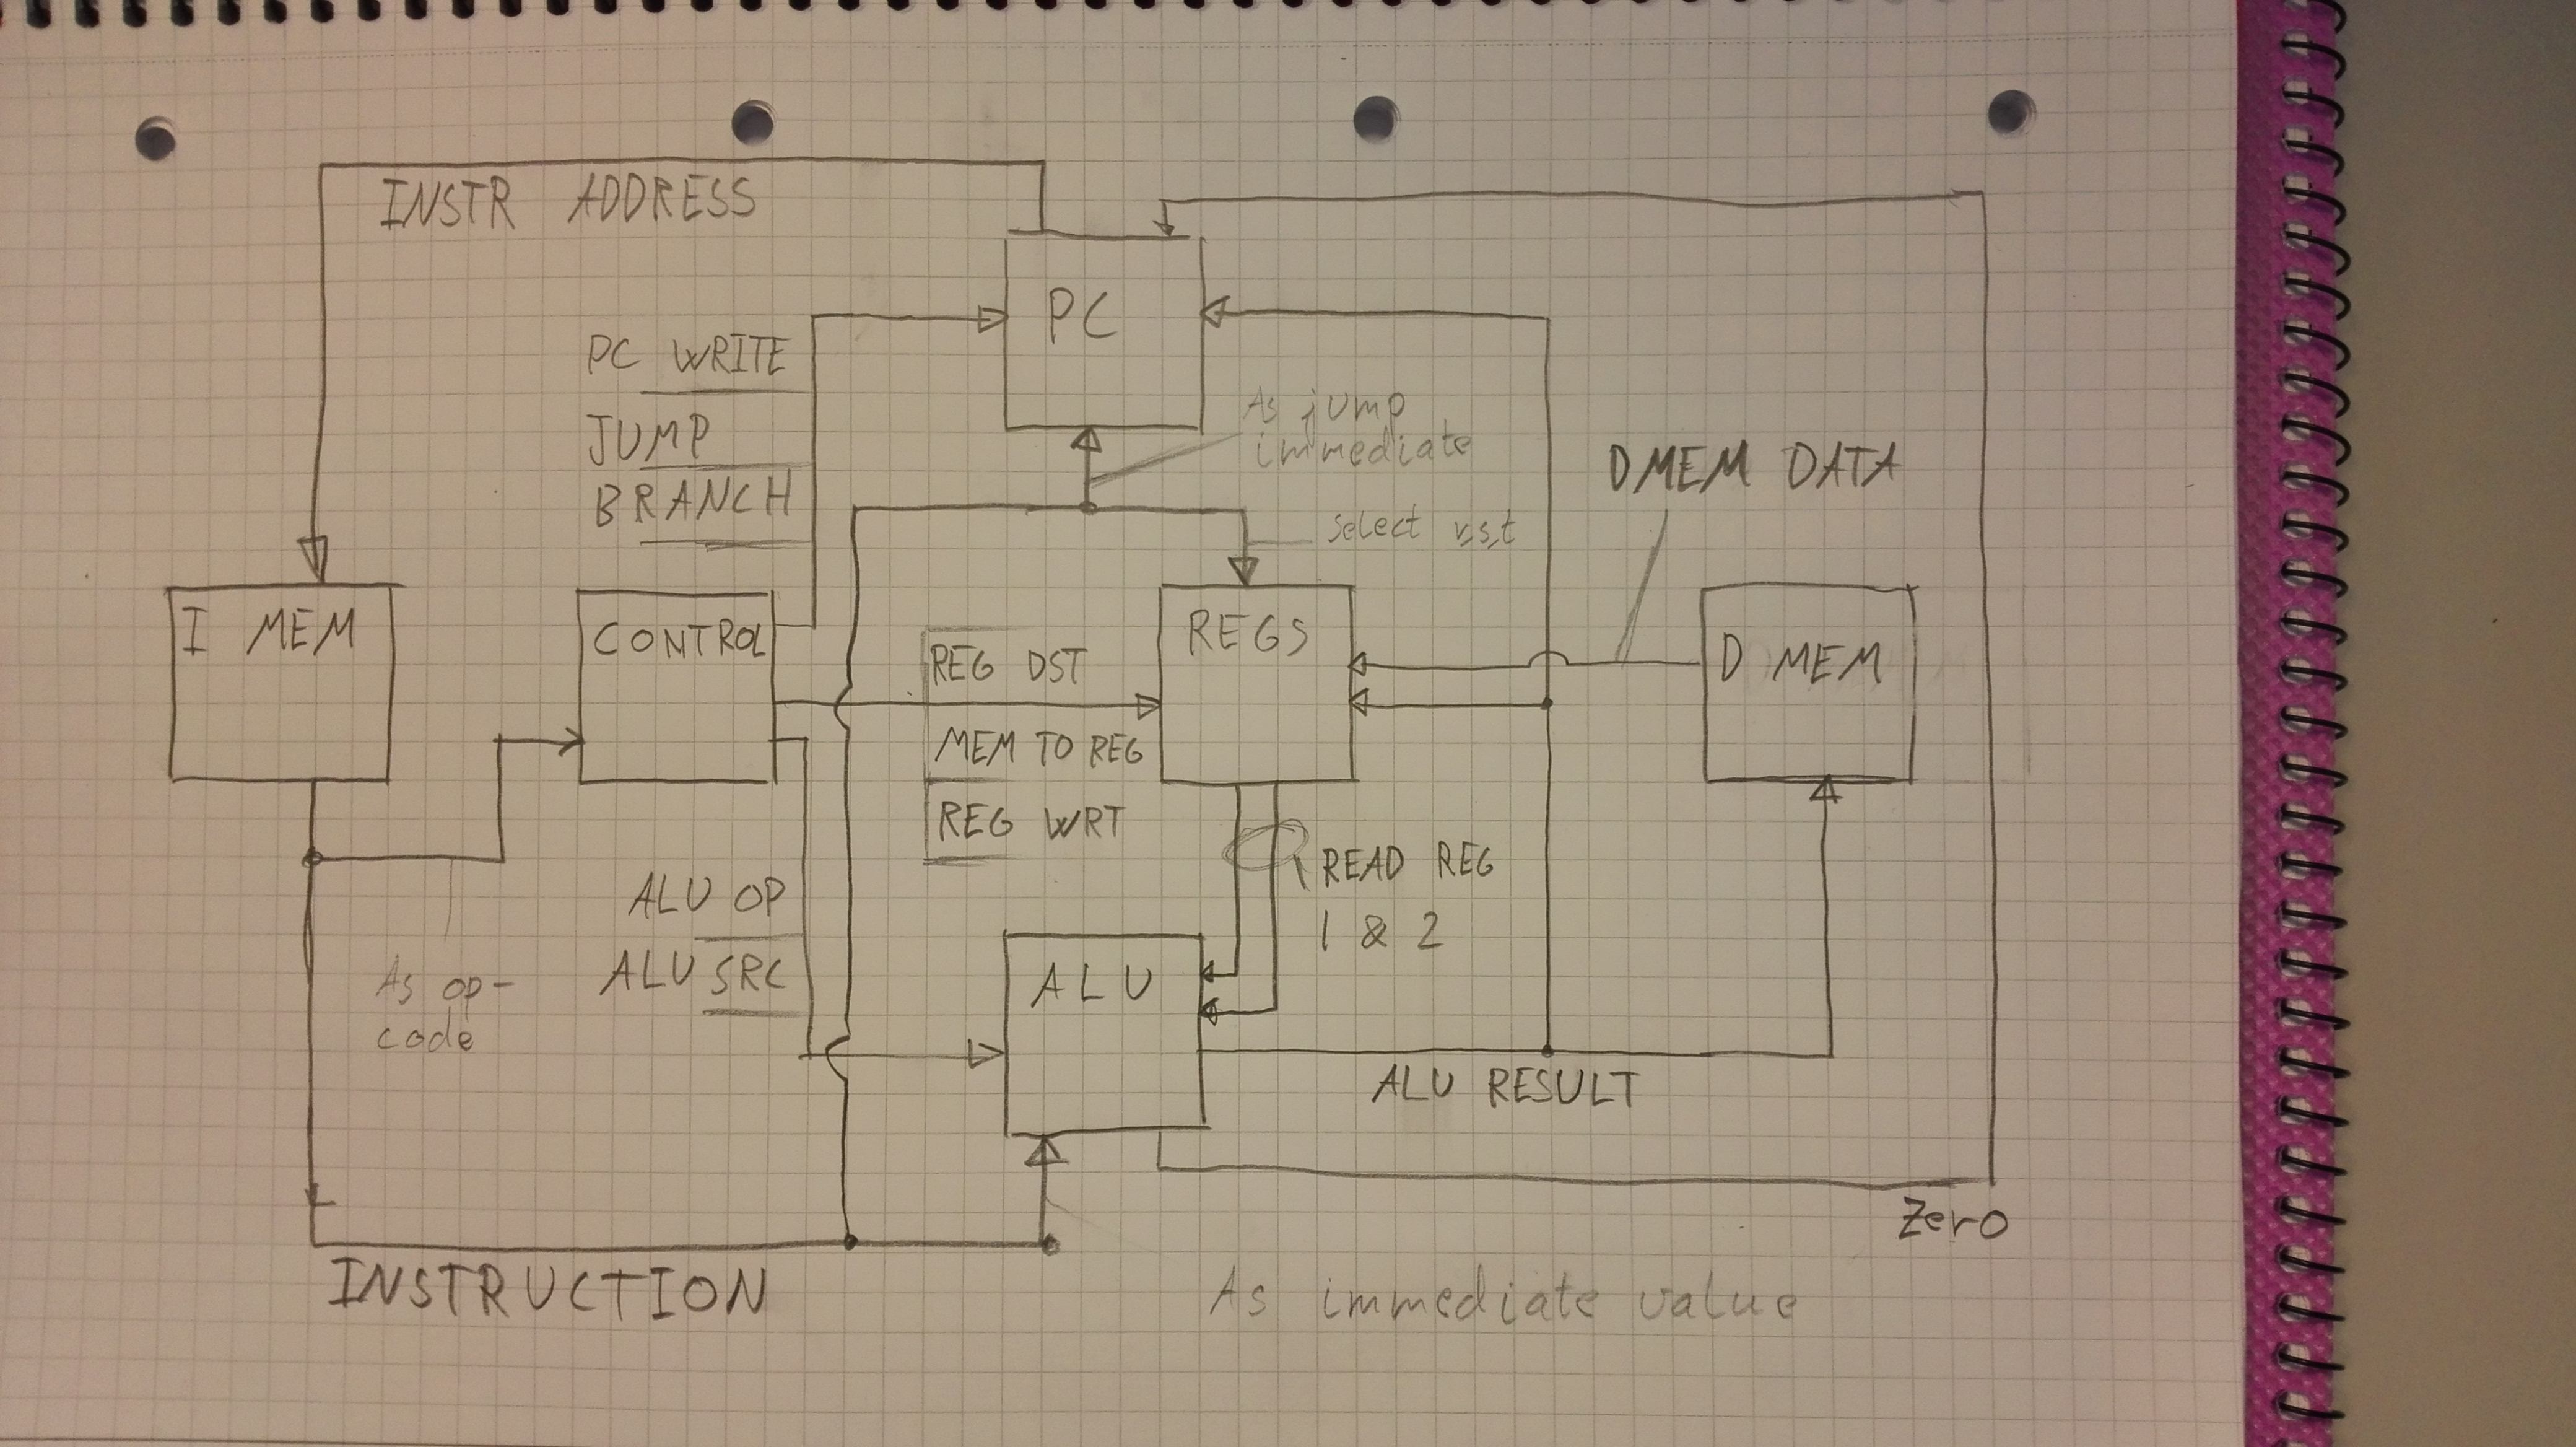
\includegraphics[width=\linewidth]{img/toplevel.jpg}
    \caption{Top level architecture sketch.}
    \label{fig:toplevel}
\end{figure}

\section{implementation}
The top level sketch introduces the four modules we have implemented, along with the two memory modules which has been provided in the exercise.
These are:

\begin{description}
  \item[Control] \hfill \\
  the control unit keeps track of the state of the processor, namely fetch, execute and stall, and then issues the appropriate control signals.  
  \item[Program counter] \hfill \\
  the program counter keeps track off the address to the next instruction to be executed. It therefore handles regular increments and calculates jumps.
  \item[ALU] \hfill \\
  the heart of the processor, the ALU performs an operation issued by the control unit and outputs a result along with a zero signal which is part of the branch logic of the PC.
  \item[Register] \hfill \\
  the register bank is the short term memory of the architecture, feeding operands to the ALU, and recieving data which may be stored based on the control signals.
\end{description}

\subsection{Control module}
The job of the control module can be partitioned into two tasks.
First, it keeps track of the current state of the processor.
These states are:
\begin{description}
  \item[Offline] \hfill \\
  The initial state, not an essential part of the design. In this state the control module simply waits for the processor to go online.
  \item[Fetch] \hfill \\
  The state in which the processor requests the next instruction from the instruction memory.
  \item[Execute] \hfill \\
  After fetching an instruction, the control module reads the opcode and issues the corresponding control signals.
  If the control unit sees an instruction which loads or stores data (other than from the internal registers), it sets the next state to stall, otherwise it goes to the execute state.
  \item[Stall] \hfill \\
  In the stall state, the control unit simply waits a cycle such that the load and store operations can finish.
\end{description}

The second task for the control module is to decode the incoming instruction, and to set the appropriate control signals. These signals will be covered in the respective modules.

\subsection{Program Counter}

The program counter calculates the next address based on the current address, the branch and jump signals issued by the control module, and a zero flag, denoting the result of the current ALU result being zero.
This calculated addres is however not used directly, the only component connected to the calculated signal is the register at the heart of the PC (often simply called the PC, and even accesible as a register in some other architectures).
The output of the PC module is the value of the PC register, thus in order to get the next address the control module issues a special signal: PC write, which enables the PC register to read the address it has calculated, outputting the new instruction address the next cycle.
Since the PC is a register, it is necessary to factor in the delay associated with state, causing the updated instruction address to be updated one cycle after the PC write signal is issued.

